% 子群和正规子群
% 子群|正规子群|左陪集|同余|商群|拉格朗日定理

\pentry{群\upref{Group}}

\subsection{子群}

\begin{definition}{子群}

给定一个群$(G, \cdot)$,如果集合$G$有一个子集$H$,使得$e\in H$且$H$中的元素在运算$\cdot$下仍然封闭,那么显然\footnote{由于已经知道$(G,\cdot)$构成一个群了,群的四条公理中,结合性、单位元存在性以及逆元存在性都被满足了.}$(H,\cdot)$也构成一个群.称$H$是群$G$的\textbf{子群(subgroup)}.

\end{definition}

虽然群和子群的联系很紧密,但是我们通常还是把它们看作由完全无关的集合所构成的,只不过可以自然地应用已经存在的群运算和子集关系来定义子群的运算.这样,将已有的运算直接用在子集上,有时被称作在子集上\textbf{导出}或\textbf{诱导(induce)}了一个运算,有时也称子集上的运算是\textbf{限制在子集上的运算}.比如在定义里,群$H$的运算实际上被认为是和$G$的运算不一样,严格来说应该记为$\cdot|_H$,意思是“限制在$H$上的$\cdot$”. 但是不至于引起混淆的时候,也可以简单记为“$\cdot$”,并认为是同一个运算.

一般来说,当我们说$H$是一个子群时,强调的是$H$和$G$的关系;但如果我们说$H$是一个群,我们关心的是$H$本身作为群的性质,而没有强调它和其它群的关系.

\begin{example}{整数加群的子群}\label{Group1_ex1}
我们已经知道,全体整数配上通常的加法,能构成一个群(\autoref{Group_ex1}\upref{Group}),可以简称为“整数加群”.整数加群的集合中包括了全体整数.如果我们只取偶数,会发现偶数之间的加法和加法的逆(减法)的结果还是偶数,也就是说,全体偶数对于整数加法是封闭的,可以构成整数加群的一个子群.这个子群,我们记为$2\mathbb{Z}$.

类似地,如果取某个整数$n$的全体倍数构成集合,这个集合上的加法也是封闭的,构成子群,记为$n\mathbb{Z}$.比如说,$3\mathbb{Z}=\{0, \pm3, \pm6, \pm9, \cdots\}$.特别地,也可以把$\mathbb{Z}$本身看成是$1$的倍数构成的集合.
\end{example}



\subsection{陪集}

\begin{definition}{左陪集}

给定一个群$G$和它的一个子群$H$.从$G$中任意挑一个元素$x$出来,用它来\textbf{左乘} $H$中的每一个元素,得到一个集合$\{x, xh_1, xh_2, \cdots\}$,这里的$h_n$要取遍每一个在$H$中的元素.这个集合,也可以写为$\{xh|h\in H\}$,被叫做\textbf{子群$H$关于元素$x$的左陪集(left coset)},记作$xH$. 

\end{definition}

类似地还可以定义右陪集,不过二者选其一作为代表来研究就可以了,我们习惯上主要研究左陪集.

注意这个表示方法:$xH=\{xh|h\in H\}$.这是一种非常简洁的表达方法,可以理解成$x$逐个左乘$H$中的元素得到的集合,也可以理解成是$x$和$H$之间的一个运算,结果是另一个集合.类似地,我们也可以用群里任意两个子集(不一定要求是子群)$A$和$B$来生成一个新的子集$AB=\{ab|a\in A, b\in B\}$,就是用$A$中的每一个元素去左乘$B$中的每一个元素,得到的所有结果的集合.我们也可以把$n\mathbb{Z}$的表示方法理解为用$n$去乘全体整数所得到的集合,这个集合构成群.

如果$h\in H$,而$H$是一个\textbf{有限群},那么由于封闭性,$hH=H$.这是因为,用$h$去左乘$H$中的一切元素(包括$h$自己),那么一方面由于封闭性,运算结果还是在$H$内部;另一方面由于群运算的唯一性,每一个左乘运算都不相同.这个论断不能简单地用于无限群.

所以,如果我们用$xH$中任意元素$xh_0$来左乘$H$,得到的$xh_0H$仍然是同一个左陪集:$xH=xh_0H$. 所以我们可以用左陪集中的任何一个元素$x'$来作为代表,把这个左陪集写成$x'H$.

特别地,考察这个形式的集合:$\{e, h, hh, hhh, hhhh, \cdots\}$,那么同样地由于封闭性和运算唯一性可知,这个集合还是群$H$的一个子集.特别地,$H$的群运算限制在这个集合上能构成一个循环群(\autoref{Group_ex2}\upref{Group}).只要我们把$n$个$h$相乘的结果记为$h^n$,$n$个$h^{-1}$相乘的结果记为$h^{-n}$,那么如此生成的循环群就可以用指数的加法运算来处理了.由单个元素可以生成循环群这一概念,我们引入以下定义:

\begin{definition}{阶}
给定一个群$G$和一个$g\in G$,如果存在一个整数$n$使得$g^n=e$,那么我们称$g$是一个有限阶的元素.特别地,所有满足条件的$n$中最小的那一个,被称为$g$的\textbf{阶(order)}.如果任何整数$n$都不能使$g^n=e$,那么我们称$g$的阶数为$\infty$.
\end{definition}

有限群的元素都是有限阶的. 证明: 若 $h, \dots, h^{n} \ne e$, 那么 $e, h, \dots, h^{n}$ 这 $n+1$ 个元素必然互不相等(例如若 $h^5 = h^3$, 那么必有 $h^2 = e$). 所以当 $n$ 等于群中的元素个数时, 必定会出现某个 $h^m = e$. 证毕. 这也说明了任意元素的阶数不会超过群中元素的个数.

\begin{example}{$n\mathbb{Z}$ 的左陪集}\label{Group1_ex2}
整数加群的群运算是通常的加法,所以我们可以把元素$k$所在的左陪集记为$k+n\mathbb{Z}$.比如说,当$n$为$6$,$k$为$1$时,$1+6\mathbb{Z}=\{\cdots, -11, -5, 1, 7, 13, \cdots\}$;当$k$为$8$时,$8+6\mathbb{Z}=\{\cdots, -10, -4, 2, 8, 14, \cdots\}=2+6\mathbb{Z}$.

$6\mathbb{Z}$一共有$6$个不同的左陪集;类似地,$n\mathbb{Z}$一共有$n$个不同的左陪集.


\end{example}

\begin{example}{$3\mathbb{Z}$的子群和左陪集}\label{Group1_ex3}
$3\mathbb{Z}$虽然是$\mathbb{Z}$的子群,但是它也可以从中再分离出子群来.由于$3\mathbb{Z}$的集合是由全体$3$的倍数构成的,因此全体$6$的倍数构成的集合$6\mathbb{Z}$是$3\mathbb{Z}$的真子集,我们已经知道它构成群了.也就是说,$6\mathbb{Z}$既是$\mathbb{Z}$的子群,又是$3\mathbb{Z}$的子群,甚至还是$2\mathbb{Z}$的子群.

从\autoref{Group1_ex2}中我们知道,$6\mathbb{Z}$作为$\mathbb{Z}$的子群,有$6$个左陪集;但作为$3\mathbb{Z}$的左陪集的时候只有$\frac{6}{3}=2$个左陪集.

下图可以形象地表示$\mathbb{Z}$,$3\mathbb{Z}$以及$6\mathbb{Z}$之间的关系,一般的群和子群的关系也可以类似理解.

\begin{figure}[ht]
\centering
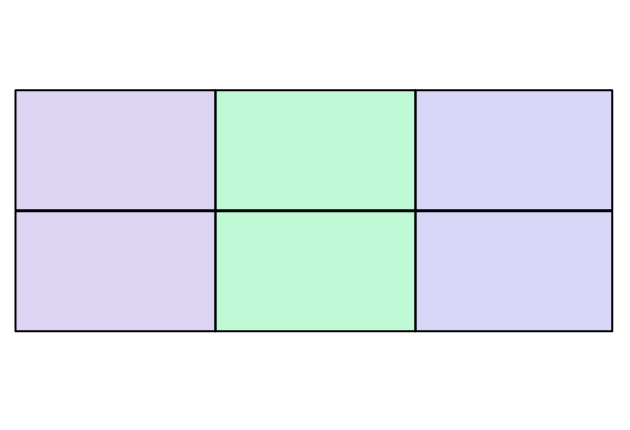
\includegraphics[width=5cm]{./figures/Group1_1.png}
\caption{子群和陪集的示意图.整张图表示$\mathbb{Z}$本身;中间的两个绿色区域表示$3\mathbb{Z}$,左边的两个紫色区域表示$1+3\mathbb{Z}$而右边的两个紫色区域表示$2+3\mathbb{Z}$;中间上面的绿色区域表示$6\mathbb{Z}$,而下面的绿色区域表示$3+6\mathbb{Z}$,剩下的四个紫色区域分别表示$6\mathbb{Z}$ 的另外四个左陪集.} \label{Group1_fig1}
\end{figure}

在这个图中可以清楚地看到,$3\mathbb{Z}=6\mathbb{Z}\cup(3+6\mathbb{Z})$.这很容易理解,因为$3$的倍数无非两种情况,$6$的倍数或者$6$的倍数再加$3$.

\end{example}

左陪集的意义是将群划分成互不相交的子集,这是一个等价类划分,也就是说,“$x$和$y$属于同一个左陪集”是一个等价关系\upref{Relat}.于是我们有了如下定理: 

\begin{theorem}{}\label{Group1_the1}

左陪集划分是一个等价类划分.

\end{theorem}

\textbf{证明}:

给定一个群$G$,两个元素$x, y\in G$,再给定它的一个子集$H$,那么“$y$在左陪集$xH$中”的等价表述,可以是“$y\in xH$”;在这个属于关系两边同时左乘一个$x^{-1}$,还能得到更常用的等价表述:$x^{-1}y\in H$\footnote{如果你不理解为什么可以像解方程一样两边同时乘以一个元素,请再琢磨琢磨上文中$xH$的定义是什么.}.

我们用最后这个等价表述来检查,“在同一个左陪集中”这一关系,是否是等价关系.
\begin{itemize}
\item 自反性:对于任意的$x\in G$,由于$e\in H$,故显然有$x=xe\in xH$.因此$x$和自己在同一个左陪集中.
\item 对称性:如果$x^{-1}y\in H$,由于$H$是个群,故$y^{-1}x=(x^{-1}y)^{-1}\in H$.因此$x$也在左陪集$yH$中.对称性还说明,如果$y$在$xH$中,那么$x$也在$yH$中,因此这两个表述可以合二为一为“$x$,$y$在同一个左陪集中”.
\item 传递性:如果$x^{-1}y\in H$,$y^{-1}z\in H$,那么由于$H$的封闭性,$(x^{-1}y)(y^{-1}x)\in H$,拆开括号后得到$x^{-1}z\in H$. 因此$z$也在$xH$中.
\end{itemize}

到此,我们证明了“在同一个左陪集中”是一个等价关系.由这个等价关系划分的左陪集,是一种等价划分,左陪集彼此互不相交.

\textbf{证毕}

\begin{definition}{同余}
对于群$G$和其子群$H$,如果$x, y\in G$满足$x, y$在同一个左陪集中,那么我们称$x, y$ \textbf{模$H$同余}\footnote{对比整数\upref{intger}中的同余概念.两个“同余”有什么联系吗?}.
\end{definition}

知道了左陪集是等价类,我们很容易发现群的一个优美的结构.在集合论中,子集的基数\upref{Set}可以是任意的,只要它小于等于原集合的基数就可以;但是子群的阶却必须能够整除原群的阶.这就是群论的\textbf{拉格朗日定理(Lagrange's Theorem)}:

\begin{theorem}{拉格朗日定理}\label{Group1_the2}

给定群$G$,如果$H$是$G$的子群,那么$|H|$可以整除$|G|$.

\end{theorem}

\textbf{证明}:

假设$x\in G$.根据$xH$的定义,$|xH|\leq|H|$. 又由群运算的唯一性,这个不等式应该取等号:$|xH|=|H|$.所以每个左陪集的基数都一样大.

左陪集彼此不相交,每个元素$x$都属于左陪集$xH$,因此$|G|$等于各个左陪集的基数之和,也就是$|H|$的倍数.

\textbf{证毕}

\subsection{正规子群}

在上文中,我们在群上定义了元素和子集间、子集和子集间的运算,还知道了左陪集是一种等价类划分.假设我们有群$G$和它的子群$H$,能不能用$H$的左陪集当元素,构成一个集合,并在上面定义一个和$G$的运算相关的群运算呢?

最直接的想法,就是直接进行左陪集之间的运算:对于左陪集$A$和$B$,有$AB=\{ab|a\in A, b\in B\}$. 但是一般来说,如果$G$的运算不是可交换的,我们这样算出来的$AB$甚至不一定是一个左陪集,那么这个左陪集之间的运算甚至不满足封闭性,自然不能是个群运算了.

如何让左陪集之间的运算满足封闭性呢?

假设我们有$x, y\in G$,它们对应的左陪集分别是$xH$和$yH$.由于$xH=\{xh_1|h_1\in H\}$,$yH=\{yh_2|h_2\in H\}$, 那么根据定义有:$xHyH=\{xh_1yh_2|h_1, h_2\in H\}$.每一个$xh_1yh_2$都在左陪集$xh_1yH$中,我们希望每一个$h_1$对应的$xh_1yH$都是同一个左陪集.

在\autoref{Group1_the1} 的证明中我们提到了一个判断两元素是否在同一个左陪集中的方法.现在假设$xh_1y$和$xh_2y$在同一个左陪集里,应用判断方法得到:$(xh_1y)^{-1}(xh_2y)\in H$.由于$(xh_1y)^{-1}=y^{-1}h_1^{-1}x^{-1}$,我们有:$$y^{-1}h_1^{-1}x^{-1}xh_2y\in H$$
也就是说$$y^{-1}h^{-1}_1h_2y\in H$$

由于这里的$y$是$G$中任意元素,$h_1$和$h_2$是$H$中任意元素,故我们要求$y^{-1}Hy\subset H$对于任何$y\in G$都成立, 其中 $y^{-1}Hy = \qty{y^{-1}h_i y|h_i \in H}$.巧的是,让$H$满足了这个要求之后,封闭性就满足了.

\begin{exercise}{}\label{Group1_exe1}
证明:对于群$G$和它的子群$H$,如果$H$满足对于任意的$g\in G$,都有$g^{-1}Hg\subset H$, 那么对于任意的$x, y\in G$,$xHyH$中的元素都在同一个左陪集中.
\end{exercise}

\begin{corollary}{}\label{Group1_cor1}
由于群运算的唯一性,从$g^{-1}Hg\subset H$我们还可以推知$|g^{-1}Hg|=|H|$,因此所需要的条件等价于$g^{-1}Hg=H$, 即 $Hg = gH$, 也就是左陪集等于右陪集.
\end{corollary}

满足\autoref{Group1_cor1}中条件的子群,被称作\textbf{正规子群(normal subgroup)}.我们把“$H$是$G$的正规子群”简记为$H\triangleleft G$或$G\triangleright H$.

现在我们考察一下,如果$H$满足了条件,那么在左陪集的集合中通过$G$的运算而导出的集合间的运算,是不是一个群运算.
\begin{itemize}
\item 封闭性:由\autoref{Group1_exe1}知,该运算有封闭性.
\item 结合性:由于$G$的运算具有结合性可知,设$x, y, z\in G$,那么$(xh_1yh_2)zh_3=xh_1(yh_2zh_3)$对任意的$h_n\in H$都成立,故而$(xHyH)zH=xH(yHzH)$成立.
\item 单位元存在性:$H$就是单位元.
\item 逆元存在性:$xHx^{-1}H=HH=H$.
\end{itemize}

这样一来,在左陪集的集合上也诱导了一个群运算,构成了一个群.我们把这个群叫做群$G$模去正规子群$H$的\textbf{商群(quotient group)},记作$G/H$.由拉格朗日定理(\autoref{Group1_the2})的证明过程可知,$|G/H|={|G|}/{|H|}$.

\begin{example}{$\mathbb{Z}$的正规子群和商群}\label{Group1_ex4}
$n\mathbb{Z}$是$\mathbb{Z}$的正规子群,这对任何$n$都成立.证明很简单,因为$\mathbb{Z}$是交换群,所以元素位置可以自由互换,因此$g^{-1}Hg=g^{-1}gH=H$对任何\textbf{子集}都成立,因此交换群的子群都是正规子群.

考虑$\mathbb{Z}$模去$3\mathbb{Z}$得到的商群,我们记为$\mathbb{Z}/3\mathbb{Z}=\mathbb{Z}_3$. 这个商群一共有$3$个元素,每个元素都是一个左陪集:$0+3\mathbb{Z}=3\mathbb{Z}=\{\cdots, -6, -3, 0, 3, 6, \cdots\}$,$1+3\mathbb{Z}=\{\cdots, -5, -2, 1, 4, 7, \cdots\}$和$2+3\mathbb{Z}=\{\cdots, -4, -1, 2, 5, 8, \cdots\}$. 换句话说,集合$\mathbb{Z}_3=\{3\mathbb{Z}, 1+3\mathbb{Z}, 2+3\mathbb{Z}\}$.

注意,虽然$\mathbb{Z}_3$的元素是集合,我们仍然要把它们看成一个个的元素.事实上,$\mathbb{Z}_n$的群结构和一个有着$n$个数字的钟表(\autoref{Group_ex2})是一模一样的,因此我们也用$\mathbb{Z}_n$来表示循环群. 

\end{example}

\begin{example}{置换群和交错群}\label{Group1_ex5}
我们知道,置换群$S_n$(\autoref{Group_ex3})是$n$个元素的变换所构成的群.为了简洁地表达变换,我们可以用以下记号:

$(1,2,3)$表示一个变换,它是将$1$号桶中的球放入$2$号桶,$2$号桶中的放入$3$号桶,$3$号桶中的又放入$1$号桶.显然,$(2,3,1)$表示的是同一个变换.$(1,2,3)(4,5)$表示的是先进行$(1,2,3)$变换,再进行$(4,5)$变换.显然,这两个变换没有涉及相同数字,所以它们是彼此分离的,可以交换:$(1,2,3)(4,5)=(4,5)(1,2,3)$.

如果两个变换有相同数字,那么我们可以把它们合并为一个括号:$(1,2)(2,3)$代表先“把$1$号桶中的球放入$2$号桶,$2$号桶中的放入$1$号桶”,再“把$2$号桶中的球放入$3$号桶,$3$号桶中的放入$2$号桶”, 最终结果是“$1$号桶中的球放入$3$号桶,$2$号桶中的放入$1$号桶,$3$号桶中的球放入$2$号桶”,也就是说,$(1,2)(2,3)=(1,3,2)$.注意$(1,2,3)\not=(1,3,2)$.

只涉及到两个元素之间的变换显然是最简单的,我们称之为\textbf{对换}.一切变换都是由若干个对换相乘(复合运算)得到的.可以证明\footnote{见\autoref{GroupP_ex1}.},每进行一次对换,桶中球的“逆序数”的奇偶性会改变.初始状态下的逆序数是$0$,一个偶数;因此如果一个变换可以被奇数个对换组合得到,那么这个变换会使得桶中球的逆序数变成奇数,这个变换就叫做奇变换;同样地,偶数个对换组合得到的变换称为偶变换,它会使得桶中球的逆序数仍为偶数.

偶变换之间的复合仍然能得到偶变换,因此全体偶变换构成置换群$S_n$的一个子群,称为\textbf{交错群(alternating group)},记为$A_n$.交错群是置换群的一个正规子群,元素数量是置换群的一半——也就是说,$|S_n/A_n|=2$对任何$n$都成立.


\end{example}

\subsection{小结}

对于任何群$G\triangleright H$,所有左陪集的元素数量都是$|H|$,包括$H$本身.这些左陪集彼此没有交集,但群$G$是所有左陪集的并集,我们由此得到了拉格朗日定理,揭示了一个任何群都具有的简洁的结构特征.商群$G/H$的元素数量,正是$G$和$H$的元素数量的商.

当子群$H$满足,对于任意的$g\in G$都有$g^{-1}Hg=H$时,$H$就成了一个正规子群.只有正规子群才能生成商群;非正规的子群划分出来的等价类,按照二元关系\upref{Relat}中提到的方法构成的商集,却并不能用$G$的运算来导出一个群运算.当然,你也可以把这个商集看成和$G$完全无关的集合,给它独立定义一个群运算,但那样这个群就和$G$没有一点关系了,不能叫做$G$的商群.

$G/H$的群运算是$G$的运算导出来的,所以继承了$G$中很多相似的性质;但是$G/H$把同一个左陪集中各个元素的差别都抹去了,相当于一个简化版的$G$.所以说,商群继承了原群的部分特征,但是没有完全继承.

接下来当我们讲到群之间的映射的时候,商群与原群“似而不同”的结构非常重要.





